\section{Introduction}
The objective of this project is to solve the following problem statement:

How can one distribute a set of students over a set of project groups in an optimal way?

Teachers face this question every time a new semester start, when they have to distribute the newly enrolled students over project groups. Our aim is to make this easier for the teachers by providing an open and simple to use platform for distributing students over groups.

We can break down this main problem into various sub-problems. Two fundamental sub-problems we already address here, and reference to in later sections. These are:

\begin{itemize}
	\item What is an optimal distribution?
	\item How do we reach this distribution?
\end{itemize}

This first question is non-technical, but pedagogical. This is not our area of expertise, so we relied on literary study to find an answer to this question.

The second question is more in the machine learning area. This problem is in general an NP-complete problem (as shown by E. Ronn~\cite{ronn1990np}): brute-forcing an optimal solution would involve evaluating all possible assignments, which makes it unfeasible even for small problem sizes.  To illustrate: even for medium sized courses (like Internet of Services) with an estimated 30 students and 6 equally sized groups, there are approximately $5\cdot 10^{26}$ possible distributions
\footnote{
If we start assigning first for group 1 place 1, then group 1 place 2, etc., then group 2 place 1, etc., we have $30!$ possibilities, but many are doubles. To be precise, there are $6!$ ways to order groups (all cause doubles), and per group $5!$ ways to order the students in the group (all cause doubles). That means that there are $\frac{30!}{6! \cdot 6 \cdot 5!} = 5\cdot 10^{26}$ unique ways to distribute 30 students over 6 groups.
}
. For a computer that can test a billion combinations per second, it would take over 16 billion years to test these combinations. This estimate is just a back-of-the-envelope calculation, but it illustrates that we need a more efficient way to search.

We take a heuristic approach by trying to optimize an objective function with taboo search. The resulting solution might not be globally optimal, but it should be close to optimal and at least better than a random assignment.

Our objective is to design and implement a matching algorithm for assigning students to project groups based on various constraints and optimization criteria, e.g. even distribution of skills, group diversity, student preferences for groups and friends/preferred partners.

The design of our algorithm is based on and similar to the solution proposed by H{\"u}bscher~\cite{hubscher2010assigning} with some modifications and extensions. In the referenced paper, he describes both the pedagogical and technical aspect of how to distribute students over groups.

\section{Current solutions}
This project was created to replace the current solution of first come first serve (FCFS) approach being handled in the Internet of Services course. This solution was not optimal since it is a mandatory course for a select number of students and an elective for the rest. So if the mandatory students were not the first to sign up they were forced into a group which may not suit their skills. Since there is a number of groups with a different range of skills requirements and a large number of students each with a unique skill set, FCFS could end up matching students to groups where they do not meet the requirements.

Also, giving mandatory students first choice would give them an unfair advantage over other students and might put non-mandatory students in suboptimal groups.

Seeing these obstacles and experiencing them ourselves, we wanted to find a solution that takes into account the student's group preferences and the skill set requirements of the group to determine an optimal solution without excluding any of the mandatory students. Our approach was to create a tool that integrates with ISIS for a smooth application process.

\section{Requirements}
The following list documents requirements we had during the implementation of the project:

\begin{itemize}
	\item The distribution algorithm must be transparent (e.g. open source).
	\item Students that mandatorily follow the course must be assigned to a group.
	\item Except for the previous requirement, mandatory students and non-mandatory students are treated equally. Mandatory students do not get first pick.
	\item The resulting distribution is stable, meaning that no two students want to switch groups
	\footnote{This requirement has been adapted: the supervisor can set global weights in such a way that this constraint is violated. Instead, the distribution is stable in the sense that no single switch results in a higher overall value of the objective function. Only if the supervisor does not change the default settings, we can still guarantee the original constraint of stable pairs.}.
	
	\item Teachers can register new courses.
	\item Teachers can set the following settings for the course:
		\begin{itemize}
			\item A name, semester
			\item The groups in the course
			\item Important skills for this course
		\end{itemize}
	\item Teachers can start a distribution. Optionally, they can then change parameters and re-start the distribution.
	
	\item Students can enroll for courses.
	\item Students can set the following parameters for the algorithm:
		\begin{itemize}
			\item Their friends, chosing from a list of enrolled students.
			\item How much they like each group, on a scale of 1 to 10.
			\item What they find more important: topics (groups) or friends. This is be on a 1 to 10 scale, not binary.
		\end{itemize}

	\item Authentication is be done through ISIS, so all and only TU Berlin students can enroll.
	\item The information must be confidential: only the student and possibly the supervisor can see a student's settings
\end{itemize}

\section{Algorithm}
\subsection{Tabu Search}
Tabu search is a pluggable heuristic search algorithm that can be successfully applied as a basis for many domain-specific optimization problems~\cite{glover2003handbook, glover1997tabu, hubscher2010assigning}. Since this is a heuristic approach, it can not guarantee that a globally optimal solution will always be found, but it will always find at least a local optimum of the objective function.

The basic idea of the search routine is that it climbs towards a local maximum and keeps a limited number of traversed states as history, in order to reduce the memory requirements of the program. The history is then used in a domain-specific way to prohibit (make tabu) similar states to those already visited, in order to keep exploring the search space instead of revisiting old solutions. Also, aspiration criteria have to be defined for lifting this restriction whenever it would prevent the algorithm from finding a better solution. The last component of tabu search is to define transitions (moves) between different states in the domain and an objective function to evaluate those states, that will be maximized by the algorithm.

\subsection{Tabu criteria}
We considered two options for the tabu criteria. The first one is to keep timestamps for every student that track the latest movement. Then moving a student would be prohibited for the next $n$ steps. This is the strategy used by R. H{\"u}bscher~\cite{hubscher2010assigning}. However, this has have a prohibitive effect on dropping and filling groups (see moves below), because these moves involve a whole set of students. Thus, if even one of these students had been moved in any of the previous $n$ steps, the dropping would be an illegal move.

The other option which we use in the final implementation, is to build a bounded tabu queue that contains the latest $n$ moves and prohibits similar moves, e.g. swapping the same 2 students (for a full list of moves, see section~\ref{sec:moves}).

\subsection{Objective Function}
This section explains in more detail the composition of the objective function that the matching algorithm tries to maximize.

First, let us define the following notations:

$I_G$ : Index of group IDs\\
$I_S$ : Index of student IDs\\
$G = \{ G_i | i \in I_G \}$ : Set of groups\\
$S = \{ S_i | i \in I_S \}$ : Set of students\\
$K^*$ : Set of all skills\\
$K_g \subseteq K^*$ : Set of global skills (per course)\\
$K = \{ K_i | i \in IG, K_i \subseteq K^* \}$ : Set of skills per group\\
$M = \{ M_{sk} | s \in I_S, k \in K^* \}$ : Skill matrix (sparse)\\
$P = \{ P_{sg} | s \in I_S, g \in I_G \}$ : Preference matrix (sparse)\\

\subsection{Components}
So far we have the following components to the objective function out of the box. More can be added later on. Every component is calculated separately over the current assignment, and then the values are combined into a total score, by multiplying them with the global weights provided in the algorithm configuration. A global weight of 0 will turn off the respective criterion altogether.

Note that some criteria are global (i.e. calculated over the whole assignment, e.g. distribution in a diverse way) whereas others are local (i.e. calculated per student, e.g. friends of a student). The objective function is well defined only when a single global criterion is used. On the other hand, local criteria allow for specifying fine grained per student weights to improve the performance of the solver.

\subsubsection{Maximally Diverse \small{(global)}}
Optimizes for groups with maximal diversity with respect to available skills. The assumption here is that knowledge sharing between peers improves with increasing difference in experience and expertise across subjects. Note that this is a global criteria. Only one of those should be used at a time.

\subsubsection{Evenly Skilled \small{(global)}}
Optimizes for groups with evenly distributed skills. The assumption here is, that in order to maximize the learning objective, all relevant skills in the groups need to be well represented. In this way, students are likely to pick up the skills that the course was designed to convey. Note that this is a global criteria. Only one of those should be used at a time.


\subsubsection{Friends and Foes \small{(local)}}
We also want to allow students to specify friends, with which they would like to be in the same group. For completeness, we show the formula that works for friends and foes, since the algorithm supports it, but the frontend does not expose this function.

$$f(s_1, s_2) = 
\begin{cases}  
	-1 \textrm{ if s2 is a foe of s1} \\ 
	0 \textrm{ if s2 is neither friend nor foe of s1} \\ 
	1 \textrm{ if s2 is a friend of s1} 
\end{cases}
$$

$$ friendsFoes = w \cdot \Sigma_{i\in I_G} \Sigma_{s_1\in G_i} \Sigma_{s_2\in G_i} f(s_1, s_2) $$

where $w$ is the local weight of student $s_1$ on this criterion.

\subsubsection{Group Preferences \small{(local)}}
One of the classic optimization criteria for solving the assignment problem is letting students express their preferences for a group. In this implementation, we also consider this factor, but it's not a strict requirement to have stable pairs. Also, we opted for a weighted map of preferences instead of an ordered list for more flexibility. In this setup, stable pairs don't make sense any more. Note that this is a local criterion, so per student weights are supported.

$$ groupPrefs = w \cdot \Sigma_{i\in I_G} \Sigma_{s\in G_i} P_{si} $$
where w is the local weight of student s on this criterion.

\subsection{Moves}
\label{sec:moves}
In our implementation of the tabu search algorithm, we allow the following moves (transitions) between valid student-group assignments:
\begin{itemize}
	\item \textbf{Swap}: swaps two students.
	\item \textbf{Switch}: move a student to another group.
	\item \textbf{Drop}: remove a group.
	\item \textbf{Fill}: put a group of students from the waitinglist in a group.
\end{itemize}

We will now explain these moves in more detail:

\subsubsection{Swap}
Function signature:
\mint{scala}{swap(s1: Student, s2: Student)}
\begin{figure}[H]
	\caption{Swapping two students}
	\label{fig:moves_swap}
	\centering
	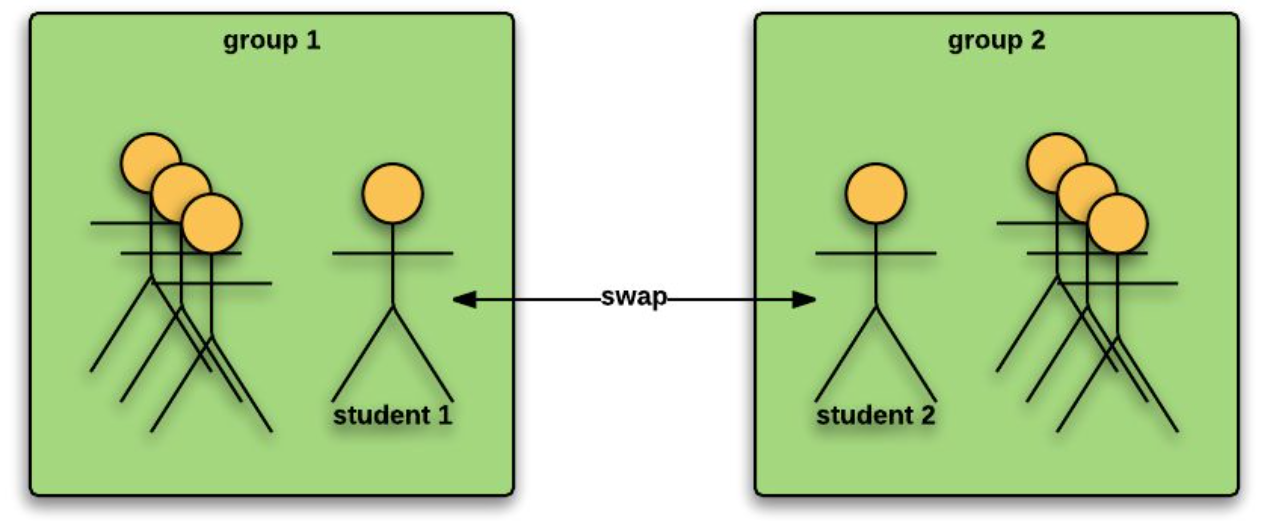
\includegraphics[width=6cm]{img/swap}
\end{figure}

Swap the (current) groups of two students; if student1 is in group A, and student2 in group B, switching them places student1 in B and student2 in A.

It is also a valid move to swap a student in a group with a student in the waiting list. However, this gives an extra requirement: in this case the course must not be mandatory for the student going to the waiting list. This constraint helps ensure that we never end up with a distribution that has mandatory students in the waiting list.

\subsubsection{Switch}
Function signature:
\mint{scala}{switch(s: Student, g: Group)}
\begin{figure}[H]
	\caption{Switching a student}
	\label{fig:moves_switch}
	\centering
	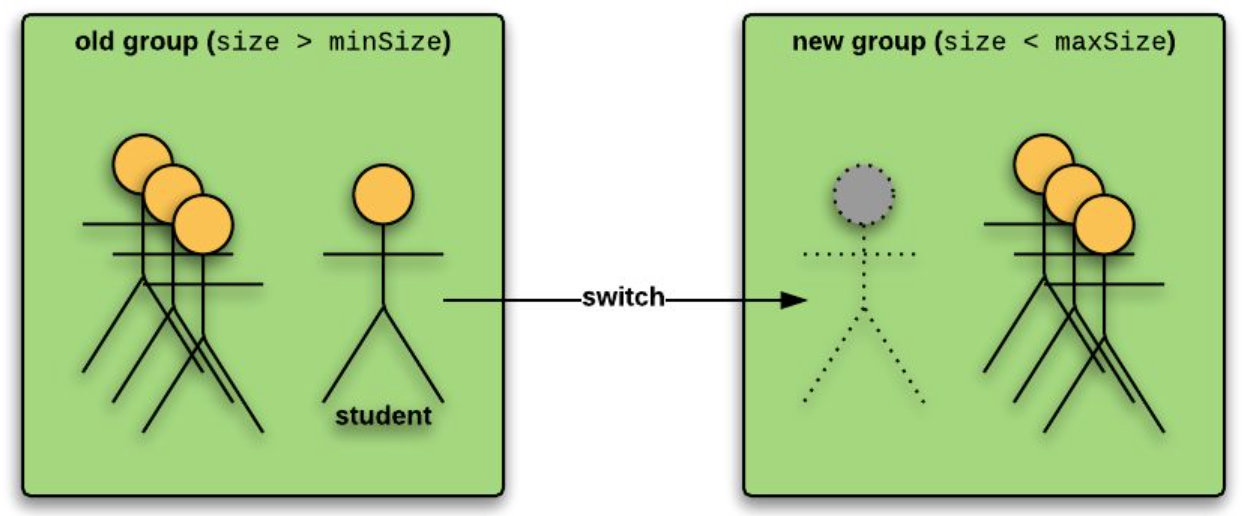
\includegraphics[width=6cm]{img/switch}
\end{figure}

Move a student from his current group to another one. After the move has been performed, the minimal and maximal group size requirements of both the old and the new group have to be fulfilled.

It is also valid to switch a non-mandatory student to the waiting list and a student from the waiting list to a regular group, but again with the restriction that the course must not be mandatory for the student. Again: this constraint helps ensure that we never end up with a distribution that has mandatory students in the waiting list.

\subsubsection{Drop Group}
Function signature:
\mint{scala}{dropGroup(g: Group)}
\begin{figure}[H]
	\caption{Dropping a group}
	\label{fig:moves_drop}
	\centering
	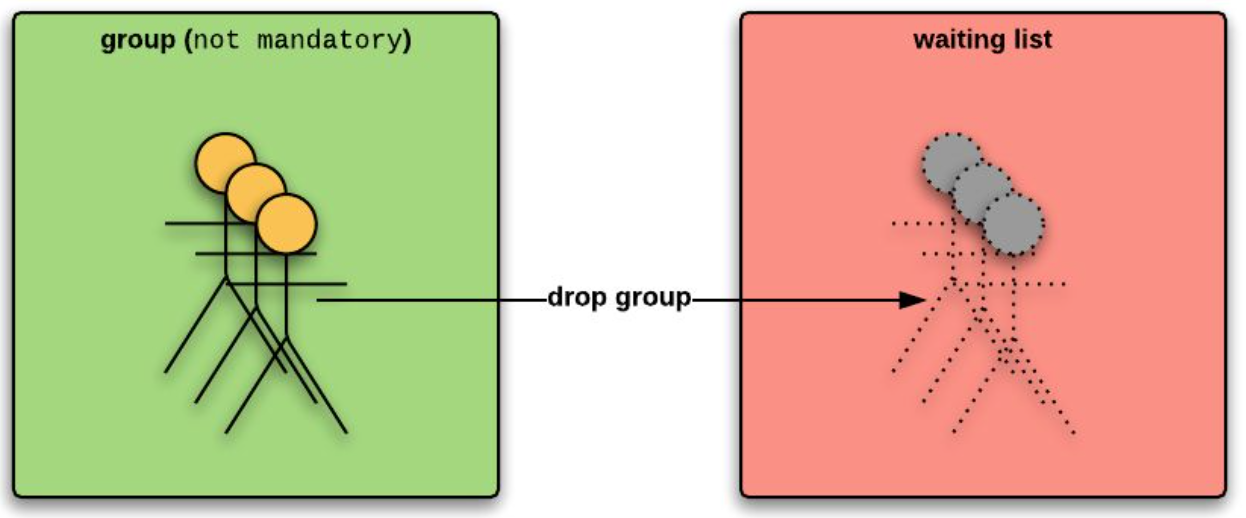
\includegraphics[width=6cm]{img/drop}
\end{figure}

Drop a group from the course and move all students currently assigned to it to the waiting list. This move is only valid if the group to be dropped is not mandatory for the course.

\subsubsection{Fill Group}
Function signature:
\mint{scala}{fillGroup(g: Group, ss: Set[Student])}
\begin{figure}[H]
	\caption{Filling a group}
	\label{fig:moves_fill}
	\centering
	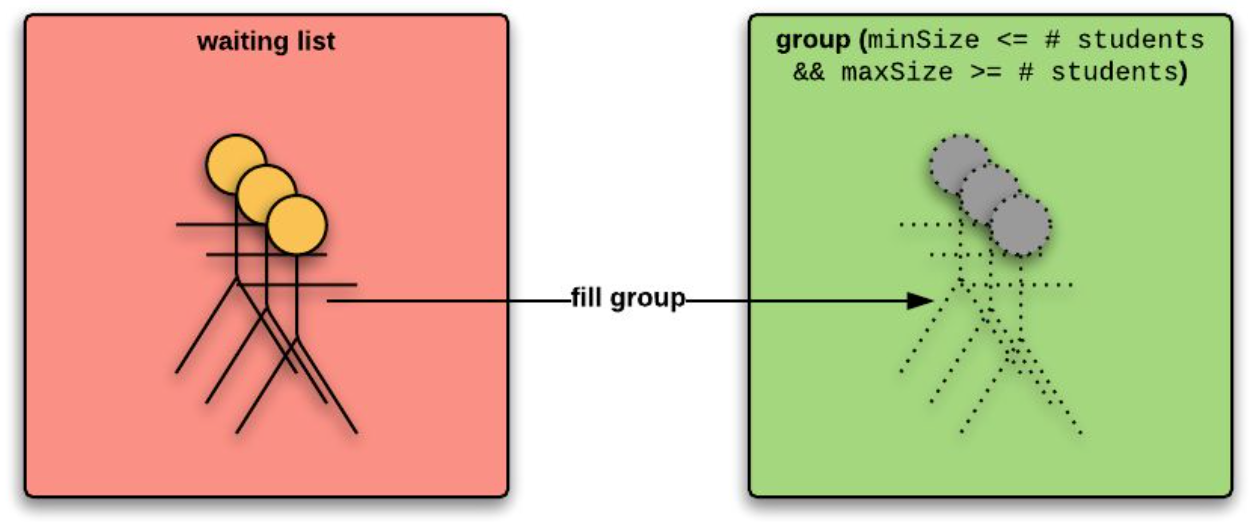
\includegraphics[width=6cm]{img/fill}
\end{figure}

Fill an empty group with a set of students from the waiting list. The number of students should be equal or greater than the minimum size and equal or less than the maximum size of the group.

It is comparable to repeated switches from the waitinglist to a group, but allows a previously dropped groups to exist again. There is one important difference: if the previously empty group has a minimum size, this method allows the group to be filled again without violating the minimum size constraint; switching checks for the minimum size constraint on every move, so a group with minimum size 5 would never be filled (since it requires 5 moves, but the first 4 are illegal).

\subsection{Models}
In this section we describe the data schema of the algorithm. Most of the input is immutable as the actual assignment is based only on references. The data has a hierarchical structure. Each instance of the algorithm deals with one course at a time, and each course is a separate run of the solver.

\subsubsection{Course}
\begin{minted}[mathescape, linenos, numbersep=5pt, frame=lines, framesep=2mm, tabsize=4, numberblanklines=true, breaklines=true]{scala}
type Course {
	jobId:        Long,
	settings:  Settings, // See the settings model
	endpoints: Endpoints, // See the Endpoints model
	students:  List[Student], // The students in this course
	groups:    List[Group], // The groups in this course
	skills:    Set[String], // List of skills, optional
	weights:   {
		maximallyDiverse: Float,
		evenlySkilled: Float,
		friendsAndFoes: Float,
		groupsPreferences: Float
	}
}
\end{minted}

\subsubsection{Settings}
The supervisor can specify settings to affect the behaviour of the algorithm. These are stored in the following model:
\begin{minted}[mathescape, linenos, numbersep=5pt, frame=lines, framesep=2mm, tabsize=4, numberblanklines=true, breaklines=true]{scala}
type Settings {
	// number of iterations without improvement before termination
	iterations: Int,
	// Number of initial positions the algorithm tries
	initialMoves: Int,
	// Number of starting points
	startingPoints: Int
	// size of the tabu list / queue
	tabuSize: Int,
	// should the algorithm optimize for diversity or equality
	diverse: Boolean
}
\end{minted}

\subsubsection{Endpoints}
The Rails server and Scala algorithm communicate asynchronously. The Rails server submits a job, and after some time the algorithm will post the results back to a special endpoint on the Rails server. This datastructure contains the URLs where the Rails server expects to receive the results.
\begin{minted}[mathescape, linenos, numbersep=5pt, frame=lines, framesep=2mm, tabsize=4, numberblanklines=true, breaklines=true]{scala}
type Endpoints {
	success: String, // URL to success endpoint on Rails server
	failure: String  // URL to failure endpoint on Rails server
}
\end{minted}

\subsubsection{Student}
\begin{minted}[mathescape, linenos, numbersep=5pt, frame=lines, framesep=2mm, tabsize=4, numberblanklines=true, breaklines=true]{scala}
type Student{
	id: Long
	name: String                  // Optional, default empty
	mandatory: Boolean            // Optional, default false
	skills: Map{String => Float}, // Optional, default empty
	weights: {
		friendsAndFoes: Float,	// Optional, default 0.5
        groupPreferences: Float   // Optional, default 0.5
	},
	// Maps groups to how much a student likes it (stored as ints referencing group ids):
	preferences: Map{Group => Float},
	// Optional (uses ints to store student ids):
	friends: List[Student], 
	// Optional, unused in the current version (stored as ints referencing student ids):
	foes: List[Student] 
\end{minted}

\subsubsection{Group}
\begin{minted}[mathescape, linenos, numbersep=5pt, frame=lines, framesep=2mm, tabsize=4, numberblanklines=true, breaklines=true]{scala}
type Group {
    id: Long,
    minSize: Int,
    maxSize: Int,
    mandatory: Boolean, // Optional, default false
    name: String,       // Optional
    skills: Set[String] // Optional
}
\end{minted}

\section{Implementation}
\subsection{High-level architecture}
The following image shows a UML diagram of the components: 
\begin{figure}[H]
	\caption{High-level architecture}
	\label{fig:high_level_architecture}
	\centering
	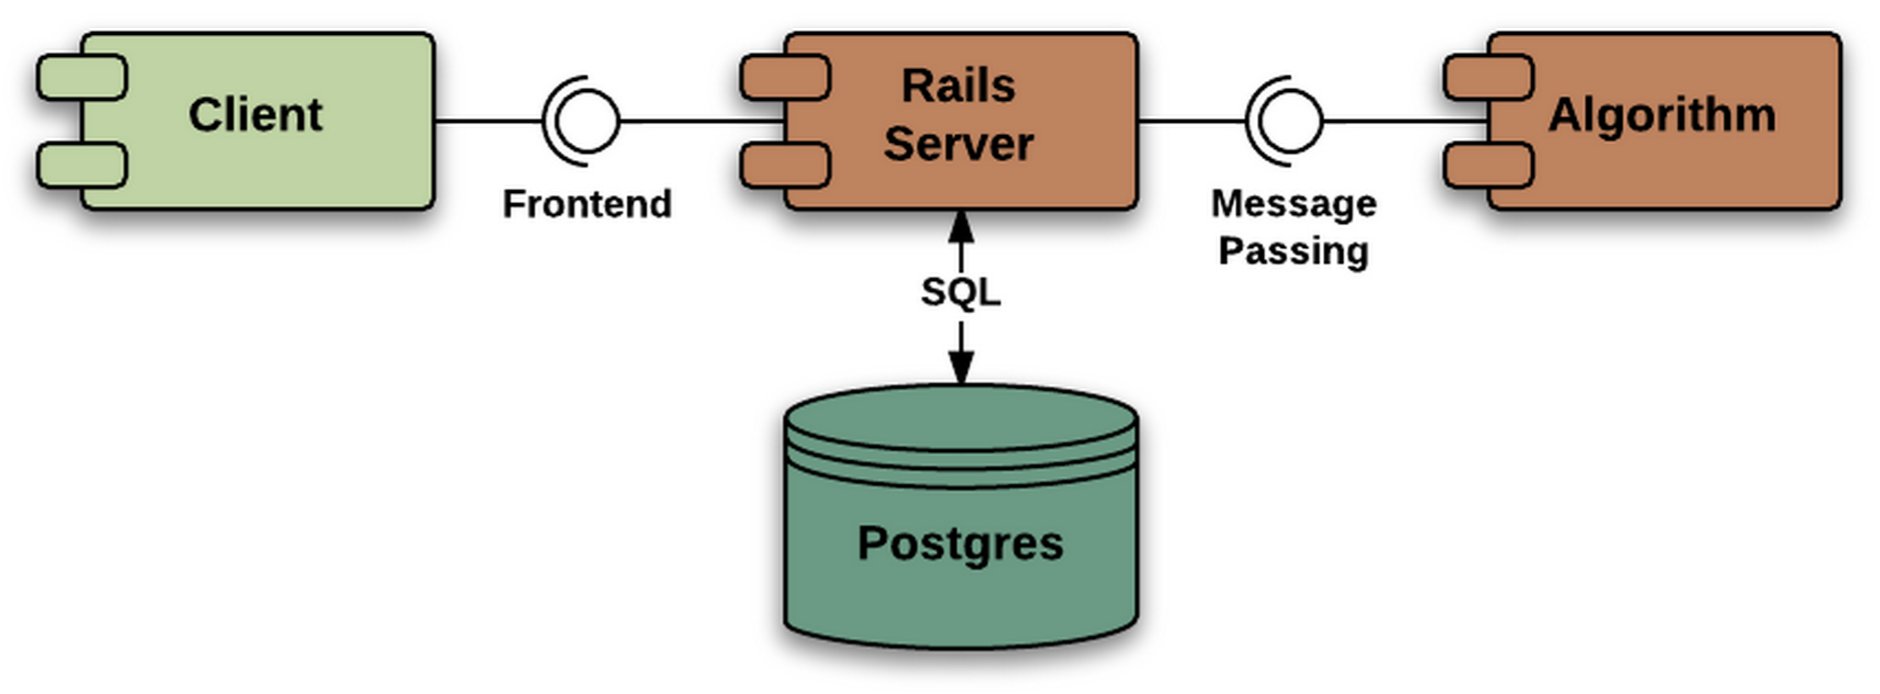
\includegraphics[width=8cm]{img/high_level_architecture}
\end{figure}

Our application has two main parts: a Rails server that processes and stores the input from the client(s). When a supervisor (client) requests a distribution to be made, the Rails server sends the data to the Algorithm server that computes a distribution and returns it to the Rails server. The Rails server stores the distribution and shows it to the clients.

This architecture allows us to have a clear separation between the simple CRUD (create, read, update, delete) application running on Rails, and the more complicated business logic in the distribution algorithm.

\subsection{Server-side}
\subsubsection{Ruby on Rails}
Ruby on Rails\footnote{\url{http://rubyonrails.org/}} (RoR) is the framework we chose for our webserver. It is a model-view-controller framework to use the Ruby programming language for displaying a site. This makes it similar to Django for Python and Spring for Java.

It was decided to use RoR because this community is very active at the time of writing. This community helps with documentation, questions and plug-ins (called gems). These plug-ins will be explained later on, and for us were a large pro for RoR, because things like authentication can be easily implemented with this. Because of the active community there are a lot of plugins available. Furthermore, it has a clear Model View Controller structure making it easy to write structured code, which helps while doing teamwork.

Furthermore, for the views we are using a language called HAML. This language is a mixture of HTML and Ruby code. It has the advantage that it works with indentations in order to define blocks does not need to be written so that an open and close tag, such as in normal HTML does have to. An example is:

\textbf{HTML}
\begin{minted}[mathescape, linenos, numbersep=5pt, frame=lines, framesep=2mm, tabsize=4, numberblanklines=true, breaklines=true]{html}
<div>
	<p>
		foo
	</p>
	<p>
		bar
	</p>
</div>
\end{minted}

\textbf{HAML}
\begin{minted}[mathescape, linenos, numbersep=5pt, frame=lines, framesep=2mm, tabsize=4, numberblanklines=true, breaklines=true]{haml}
%div
	%p foo
	%p bar
\end{minted}

\subsubsection{Phusion Passenger}
It is a web and application server design with to be robust lightweight and fast. It reduces the friction of deploying RoR apps and have an extensive number of enterprise grade features which become extremely useful in production. Some of its key features are the ability to handle more traffic(up to 4x more in RoR), its reduced need of maintenance and improved security. 

\subsubsection{Postgres}
Rails has an ORM called Active Record through which it can connect to to various databases (e.g. Postgres, MySQL, SQLite, etc.). We choose to connect it to a Postgres database, because this is a very active and widely used database. This means there are many tools that connect with the database and we can be sure of future maintenance. Also, Postgres is more performant than SQLite.
If future developers want to run a different database, they can switch without any trouble. Setting up the configuration file is sufficient, since our code is database-agnostic.

\subsection{Algorithm-side}
\subsubsection{Scala}
For the core of the algorithm we chose to work with Scala\footnote{\url{http://www.scala-lang.org/}} for a couple of reasons:
\begin{itemize}
\item It is a JVM-based language and can seamlessly interact with Java and thus we could make good use of OpenTS\footnote{\url{http://www.coin-or.org/Ots/}}, an open source tabu search implementation in Java.
\item It supports higher order functions and persistent immutable data structures, which play together nicely to ease the processing and transformation of nested data.
\item Since the algorithm implementation is stateless, we can use the rich support in Scala for multithreaded and distributed systems to easily scale it out.
\item We are familiar with Scala from our previous work.
\end{itemize}

\subsubsection{SBT}
SBT\footnote{\url{http://www.scala-sbt.org/}} naturally goes with Scala as the dependency management and build tool for the job.

\subsubsection{Spray}
Spray\footnote{\url{http://spray.io/}} is a lightweight HTTP/REST layer built with Akka\footnote{\url{http://akka.io/}} and is also easily scalable. Its features include automatic content type and error handling and composable routes, built of nested and reusable declaratives.

\subsection{Hapi on NodeJS vs. Ruby on Rails}
In this project our initial attempt to build the backend server was done with a mixture of Node.js using the Hapi framework and Bookshelf.js which is built on top of the Knex.js library for Postgres SQL. This decision was made since Node has been already proven to be able to function as a robust web server implementation, and also since it was a technology which most of the group felt very comfortable working with. When designing our database we opted for a relational database as Postgres instead of MongoDB since it fitted best with our design criteria. 

However, even though the Node community is very active and there is a lot of hype and development around it, our development process was slower than initially planned. At this point we decided to switch from Node to RoR since Rails is more of an opinionated framework and has a lot of out of the box functionality built in to speed up prototyping. Also we would get the advantage of the ActiveRecord ORM when handling nested relationships. This as opposed to implementing the relationships ourselves using Bookshelf.js library as we would have had to do in Hapi.

Once we changed our framework we split up the backend responsibilities so one team member would handle the Rails implementation while the other would fully Dockerize deployment and handle DevOps. 

\section{Deployment}
There are two ways to run the project: either by running a regular installation on the local machine or by using Docker. We added support for Docker to allow for easier deploys: if a version runs on our development computers (in Docker), then it will also run on the production server.

We recommend Docker to be used for the production, and normal installations of Rails/Postgres/SBT for development. The rationale behind this recommendation is that we tested our work on Docker, but not on every other platform.

In this section, we first give some description on how to use Docker in this specific setting. We also give some details about the virtualized networking, which may be useful for future developers.

\subsection{Starting Docker}
In this section, we show how to do a quick installation of Docker and Docker Compose, and how to build and run the images of this project. Note that this is a short (and by the time you read this possibly outdated) installation guide: for the newest installation of Docker (Compose), we refer to their site: \url{https://docs.docker.com/compose/install/}. Also, some of these commands need root permission: if you get an error, prepend the command with ``sudo", and try again.

\begin{minted}[mathescape, linenos, numbersep=5pt, frame=lines, framesep=2mm, tabsize=4, numberblanklines=true, breaklines=true]{bash}
# Install on Linux (Ubuntu)

# (If you don't have curl, first install curl)
$ curl -sSL https://get.docker.com/ | sh

# Beware: fixed version number. This one we tested on and worked for us. Future versions may have breaking changes.
$ curl -L https://github.com/docker/compose/releases/download/1.3.3/docker-compose-`uname -s`-`uname -m` > /usr/local/bin/docker-compose 
$ chmod +x /usr/local/bin/docker-compose

# If you want to run Docker as a normal user (i.e. not prepending sudo everytime)
$ sudo usermod -aG docker <your username>
# Now logout and login again to update the group changes

# Install on OSX
$ brew install docker
$ brew install boot2docker

# Download and run the project
# Fetch repository: only the first time
$ git clone https://github.com/juancroca/ios.git .

# Build containers and run the images
$ docker-compose build
$ docker-compose up -d
\end{minted}


When issuing these commands, the latest versions of the server and algorithm are fetched from Github, installed in Docker images and started. The first time one runs these commands, all dependencies have to be downloaded, which can take quite a while. After that, the cache is used and everything runs faster.

Notice that we pass a -d flag; this starts Compose in daemon mode, meaning that the process will continue after the current user has logged out.

You now have a running instance. There is one problem left: the database is not setup yet. We can use Rake to setup everything for us:

\begin{minted}[mathescape, linenos, numbersep=5pt, frame=lines, framesep=2mm, tabsize=4, numberblanklines=true, breaklines=true]{bash}
# We first enter the running Ruby instance:
$ docker exec -ti ios_ruby_1 bash

# Execute the rake command to create and setup a clean database
$ export RAILS_ENV=production
$ rake db:create
$ rake db:schema:load
\end{minted}

If, for some reason, you wish to do a restart with the existing data, just repeat the following command:

\begin{minted}[mathescape, linenos, numbersep=5pt, frame=lines, framesep=2mm, tabsize=4, numberblanklines=true, breaklines=true]{bash}
# Start the system
$ docker-compose up -d
\end{minted}

If you run this command while the old version is still running, the system will simply reboot the instance. You may experience a few seconds of downtime.

\subsection{Resetting the system}
Since loading the schema sets up empty tables, it is effectively a reset of the system. Thus, if you wish to reset the database, you can execute it again and all data will be gone. Please keep in mind that recovery is {\bf not} possible.

\begin{minted}[mathescape, linenos, numbersep=5pt, frame=lines, framesep=2mm, tabsize=4, numberblanklines=true, breaklines=true]{bash}
# We first enter the running Ruby instance:
$ docker exec -ti ios_ruby_1 bash

# Execute the rake command to setup a clean database
$ export RAILS_ENV=production
$ rake db:schema:load
\end{minted}

\subsection{Stopping Docker}
To stop docker, simply issue the following command:

\begin{minted}[mathescape, linenos, numbersep=5pt, frame=lines, framesep=2mm, tabsize=4, numberblanklines=true, breaklines=true]{bash}
$ docker-compose stop
\end{minted}

Note that this only works in the root directory of the project. Docker-compose requires the configuration files (docker-compose.yml and the Dockerfile files) to work, which it can't find if these commands are issued from another folder.

\subsection{Deploying new versions}
To fetch a new version of the server, we have to fetch and merge the new version from github:

\begin{minted}[mathescape, linenos, numbersep=5pt, frame=lines, framesep=2mm, tabsize=4, numberblanklines=true, breaklines=true]{bash}
$ git fetch && git pull
\end{minted}

To run it, execute:
\begin{minted}[mathescape, linenos, numbersep=5pt, frame=lines, framesep=2mm, tabsize=4, numberblanklines=true, breaklines=true]{bash}
$ docker-compose build
$ docker-compose up
\end{minted}

This will automatically kill any older versions that may be running and replace them with the updated versions. Also, this will automatically update the algorithm: our startup scripts always fetch the latest version.

\section{Advanced Docker usage}
This section gives an introduction on how to do some of the more complex Docker tasks.

\subsection{View running instances}
To see whether all containers are up and running:
\begin{minted}[mathescape, linenos, numbersep=5pt, frame=lines, framesep=2mm, tabsize=4, numberblanklines=true, breaklines=true]{bash}
$ docker ps
CONTAINER ID  IMAGE           ... PORTS                        NAMES
addbed0b5a9a  ios_ruby:latest ... 0.0.0.0:80->80/tcp, 443/tcp  ios_ruby_1          
91a970f6140b  postgres:latest ... 5432/tcp                     ios_db_1
\end{minted}

\subsection{Interacting with containers}
Before we continue, a fair warning: since this is the advanced way of accessing the containers, we also assume more knowledge of the reader. Accessing the system through docker exec is more aimed at developers to experiment, not for regular maintenance...

We choose not to expose SSH ports on any of the hosts for security reasons. One can, however, still access the terminal of running instances through Docker. This is only possible from the host machine. 

\begin{minted}[mathescape, linenos, numbersep=5pt, frame=lines, framesep=2mm, tabsize=4, numberblanklines=true, breaklines=true]{bash}
# Using the CONTAINER ID of a container, we can get shell access
$ docker exec -t -i addbed0b5a9a /bin/bash
# just to prove we are now in the Docker container: who am i?
root@addbed0b5a9a:/home/app/webapp# whoami
root
root@addbed0b5a9a:
\end{minted}

Alternatively, you could also use the name of the container (instead of the id):
\begin{minted}[mathescape, linenos, numbersep=5pt, frame=lines, framesep=2mm, tabsize=4, numberblanklines=true, breaklines=true]{bash}
$ docker exec -t -i ios_ruby_1 /bin/bash
\end{minted}

\subsubsection{Accessing Postgres through psql}
This section is on how to get into the psql console on the Postgres container.

Note that this time, we use the name of the container (ios\_db\_1) instead of its container id. Both versions are possible, and have the same result. Feel free to choose your favorite.

\begin{minted}[mathescape, linenos, numbersep=5pt, frame=lines, framesep=2mm, tabsize=4, numberblanklines=true, breaklines=true]{bash}
# Enter the container
$ docker exec -ti ios_db_1 /bin/bash

# Switch from root to postgres
root@91a970f6140b:/# su postgres

# Start the psql console
$ psql
psql (9.4.1)
Type "help" for help.

postgres=# \connect ios
You are now connected to database "ios" as user "postgres".
ios=# SELECT id, name, email FROM users;             
 id  |    name    |         email                
-----+------------+-----------------------
   2 | Student 1  | student1@example.com
   3 | Student 2  | student2@example.com
   4 | Student 3  | student3@example.com
\end{minted}

You can now type commands to control Postgres. Since this is (far) outside the scope of normal usage, we won't go into detail on how psql works. If you do not know how psql works, we recommend you either read a tutorial or use Google/Stackoverflow if you have questions.

To exit psql, simply do:
\begin{minted}[mathescape, linenos, numbersep=5pt, frame=lines, framesep=2mm, tabsize=4, numberblanklines=true, breaklines=true]{bash}
postgres-# \q
# Ignore this warning: it is not important (only related to psql history)
could not save history to file "/home/postgres/.psql_history": No such file or directory
$ exit
root@91a970f6140b:/# exit
# Now you're back in your normal machine
$ 
\end{minted}

\subsubsection{Accessing the Rails Console}
One of the nice tools Rails offers to developers is the Rails console. It allows you to interact with a running instance of the Rails server. You could, for example, run some debugging functions within a running instance or query data in ActiveRecord (Rails' ORM).

\begin{minted}[mathescape, linenos, numbersep=5pt, frame=lines, framesep=2mm, tabsize=4, numberblanklines=true, breaklines=true]{bash}
# Enter the Rails container
$ docker exec -t -i ios_ruby_1 bash
# Set the mode to production
root@addbed0b5a9a:/home/app/webapp# export RAILS_ENV=production
# Open the Rails console
root@addbed0b5a9a:/home/app/webapp# rails console
# Ignore messages about Pristine.
# You are now in the Rails console. You can execute commands, such as listing all users:
irb(main):001:0> User.all
  User Load (11.4ms)  SELECT "users".* FROM "users"
=> #<ActiveRecord::Relation [#<User id: 1, name: "Supervisor 1", isis_id: nil, created_at: "2015-06-28 16:53:22", updated_at: "2015-06-28 16:53:22", email: "supervisor1@example.com", encrypted_password: "", remember_created_at: nil, sign_in_count: 0, current_sign_in_at: nil, last_sign_in_at: nil, current_sign_in_ip: nil, last_sign_in_ip: nil>,....
\end{minted}

You can also interact with the models, update data, etcetera. Experienced Rails users may prefer this over changing data through the psql interface. To give a small example where we change the name of a student, consider the following:

\begin{minted}[mathescape, linenos, numbersep=5pt, frame=lines, framesep=2mm, tabsize=4, numberblanklines=true, breaklines=true]{bash}
irb(main):004:0> u = User.first
  User Load (0.8ms)  SELECT  "users".* FROM "users" ...
=> #<User id: 1, name: "Supervisor 1", ...
irb(main):005:0> u.name = 'My new name'
=> "My new name"
irb(main):006:0> u.save
   (0.6ms)  BEGIN
  SQL (3.9ms)  UPDATE "users" SET "name" = $1, ...
   (1.1ms)  COMMIT
=> true
irb(main):007:0> User.first
  User Load (0.7ms)  SELECT  "users".* FROM "users" ...
=> #<User id: 1, name: "My new name", ...
\end{minted}


Again: this document is not ment to teach you how the Rails console works. If you want to use it, we refer to the many online tutorials that explain how to work with the Rails console.

\subsection{Docker networking}
There are two ways of opening ports in Docker: opening ports internally and externally. To specify which ports are open, one can use the docker-compose.yml file:

\begin{minted}[mathescape, linenos, numbersep=5pt, frame=lines, framesep=2mm, tabsize=4, numberblanklines=true, breaklines=true]{yaml}
ruby:
  build: .
  ports:
    - "80:80"
  links:
    - db
    - scala
\end{minted}

In this example, we define the behaviour of a host labelled "ruby". It exposes port 80 to the outside world, and has access to the hosts labelled "db" (the Postgres server) and "scala" (which runs the algorithm). It cannot access all ports of db and scala, only the ports exposed by these images.

Since "outsiders" do not need direct access to the database or algorithm server, we only expose the ports of these images internally. For example, the pg host is defined by the following configuration:

\begin{minted}[mathescape, linenos, numbersep=5pt, frame=lines, framesep=2mm, tabsize=4, numberblanklines=true, breaklines=true]{yaml}
db:
  image: postgres
  expose:
    - "5432"
\end{minted}

Notice that we only specify the port Postgres uses (5432), without specifying a corresponding outer port.

\section{Continuous Integration}
We used Travis to do continous integration. Combined with Slack, this gives us feedback on our code quality on every git push. It monitors our GitHub repository and every time it detects a change, it runs test against the latest version. In Slack, this looks as following:

\begin{figure}[H]
	\caption{Slack message on Travis tests}
	\label{fig:slack_ci}
	\centering
	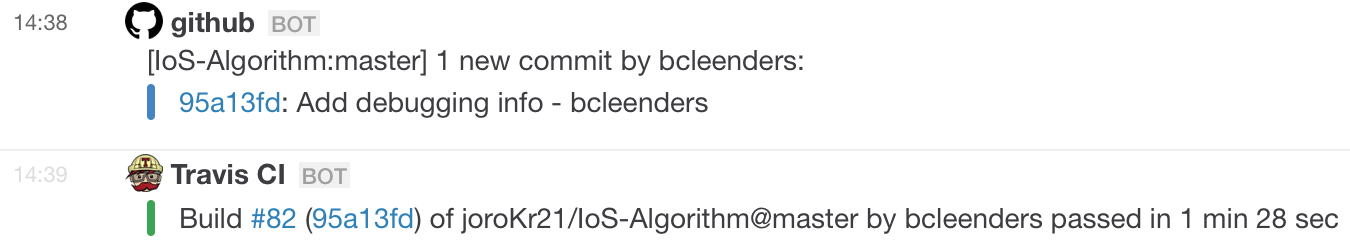
\includegraphics[width=14cm]{img/slack_ci}
\end{figure}

We agreed on the convention that in a pull-request to the master branch all tests must pass before the code is merged. Because of this you can ensure that at all times there is a working master version (or at least one that passes the tests). This method of continuous testing makes it possible to add new code and verify that all the existing code is still functioning. The continuous integration server makes it possible to deploy new code several times a day because everything is tested thoroughly.

A problem we ran into, is that Travis only runs tests for one specific language. To be able to run tests both for Scala and for Ruby, we had to split the project into two separate git repositories, with two separate Travis test suites. This did have the consequence that although each might be working separately, the combination of the two might fail without us knowing. We found no solution for this, other than doing manual tests.

\section{Result Evaluation}
TODO

TODO

TODO

TODO

TODO

TODO

\section{Group Work Evaluation}
The construction of the previously described app was not the only result expected for this course. There were other objectives like how the group is managed, how are obstacles tackled and how are decisions and compromises are made. It was undoubtedly a great learning experience, as you can see we did have some hiccups during the development of this solution. 

Initially finding the correct algorithm to solve this specific problem was not easy it involved a lot of research from some of our team members and some heated discussions. After debating several options we could finally agree on a path we all found viable.

On the other hand, on the backend server side we encounter a major bottleneck with our initial setup so we had to quickly adapt to be able to solve this problem in the expected timeframe, so that is why the change in stack occurred mid development. We were able to accomplish this due to our well-managed communication. We had a weekly face-to-face hacking day during which the entire team got together and devoted its entire time to this project.

Besides this, we started a group chat in Slack which was fully integrated with our git and continuous integration server. We had two repositories corresponding to each of the different components of the solution, this would give the team members the ability to track the project status as a whole as well as the progress of each component, we could see at all times who was developing which features and also which were completely done. 

We did notice that, as there were more and more features, it became more difficult to maintain a good overview of the exact status of every independent feature. If we had continued for a longer time and added more features, we would have had to invest (more) time in a feature tracking system.

After we felt confident with the solution we had built we ran tests comparing our implementation to a brute force solution, we found out that when having a small test dataset the results where 98\% accurate and it always found a local optimum. Even though tests with bigger datasets could not be run due to the very rapidly increasing complexity, we are confident that if this test would be feasible the accuracy of our results would not vary that much than the ones obtained in small data sets.

\section{Future Work}
In the future we would like to see some additional work done in the next areas:

\textbf{I18n}\footnote{\url{http://guides.rubyonrails.org/i18n.html}}: It would be nice if the app would take into account internalization(not only the front end), so the tool could be used in all different courses for TU Berlin where English is not the expected language. Rails is already setup to handle this kind of feature is just a matter of editing the front end and setup the proper yaml files. This tweak would also involve some work regarding the skill selection since currently we are using a predefined skillset in English.

\textbf{Integration with more services}: It would be useful to have a more advanced authentication mechanism in place when communicating with ISIS through the LTI protocol. This protocol already supports OAuth, and we would recommend to also have this type of authentication between the algorithm API and the RoR app. Versioning the algorithm API would be a good idea so it would be able to function when the json format evolves to satisfy more features.
 
\textbf{Standalone API}: Currently there are some endpoints who are able to receive a request and respond all in json format but we would like to extend this functionality so all of the endpoints are able to function this way and you can have different front end solutions built on top of the functioning RoR app.

\textbf{Extending Algorithm with more criteria}: Currently the only way we can see if a student is the correct fit for a course or not is based on the score he grants himself regarding the skillset of each group. This is a bit too subjective and if we add something like students rating each other this could improve the selection criteria on the objective function.

\textbf{Linking history}: If we integrate results of previous courses, we might be able to give a more accurate description of what students work well together. For example: at the end of the semester, students could be offered the option to rank how well they liked their other teammembers. This could then be taken into account for future distributions for next courses.